\chapter{Design}

SQAT need to handle many requests per day. Let's say we have 3000 users from School of Computer Engineering, School of Electrical and Electronic Engineering and School of Physical and Mathematical Sciences. Assume that each student will submit a request per day, which is not true because each student will submit more than one request per day in real situation. We probably need 30 seconds process one request using a server, which is reasonable because each Java project is probably made up of 10-50 files. Under perfect conditions, we need $3000 \times 30 \div 60 \div 60 = 25$ hour to complete all requests in a day (24 hour). Apparently, we need a scalable solution to handle these requests. In the following sections, we will discuss about an architecture that allows us to scale our system horizontally to handle more requests. We will also discuss about the main tool that we use to develop the software quality measurement components. We end this chapter by discussing about the architectures for the software quality measurement components and the web user interface.  

\section{Microservices}

Microservices is a software architecture style in which complex applications are composed of small, independent processes communicating with each other using language-agnostic application programming interface (API) \cite[]{martinfowler2014}. Processes that run some applications are called services. Services communicate with each other with a mechanism, such as remote procedure call. 

Before we discussed about the advantages of microservice architecture, we first discussed about another extreme of architecture design. Microservice architecture is made up of composable, small, and independent services. In contrast, monotolithic architecture is made up of multi-tier components, with components in upper tier use components in lower tier to perform some functions. If we were to develop SQAT using monotolithic architecture, we could possibly come out with a multi-tier architecture, as shown in Figure \ref{figure:SQAT_monolithic}. This architecture has three major drawbacks:

\begin{enumerate}
    \item It requires long term commitment to a particular technology stack. For example, if we choose to use Java programming language and its technology, we have to use it for anything we want to develop. If we discover a newer technology, library, or framework (in another language) in the future, we might not able to adopt them without rewriting the whole application. 
    \item It is very difficult for a developers, especially the new developers, to understand the whole application. It requires developers to learn the whole stack of technology before they can modify the application. 
    \item Scaling the application is difficult. To scale the application, we need to rent more servers to host the whole applications at each server, as shown at the bottom of Figure \ref{figure:SQAT_monolithic}. However, different application might have different resource requirements. For example, software quality measurement tools might need to CPU for more computing power and user manager might need more RAM for in-memory caching. As a result, scaling application with monolithic architecture might not result in optimal use of computing resources.
\end{enumerate}

\begin{figure}[t]
    \centering
    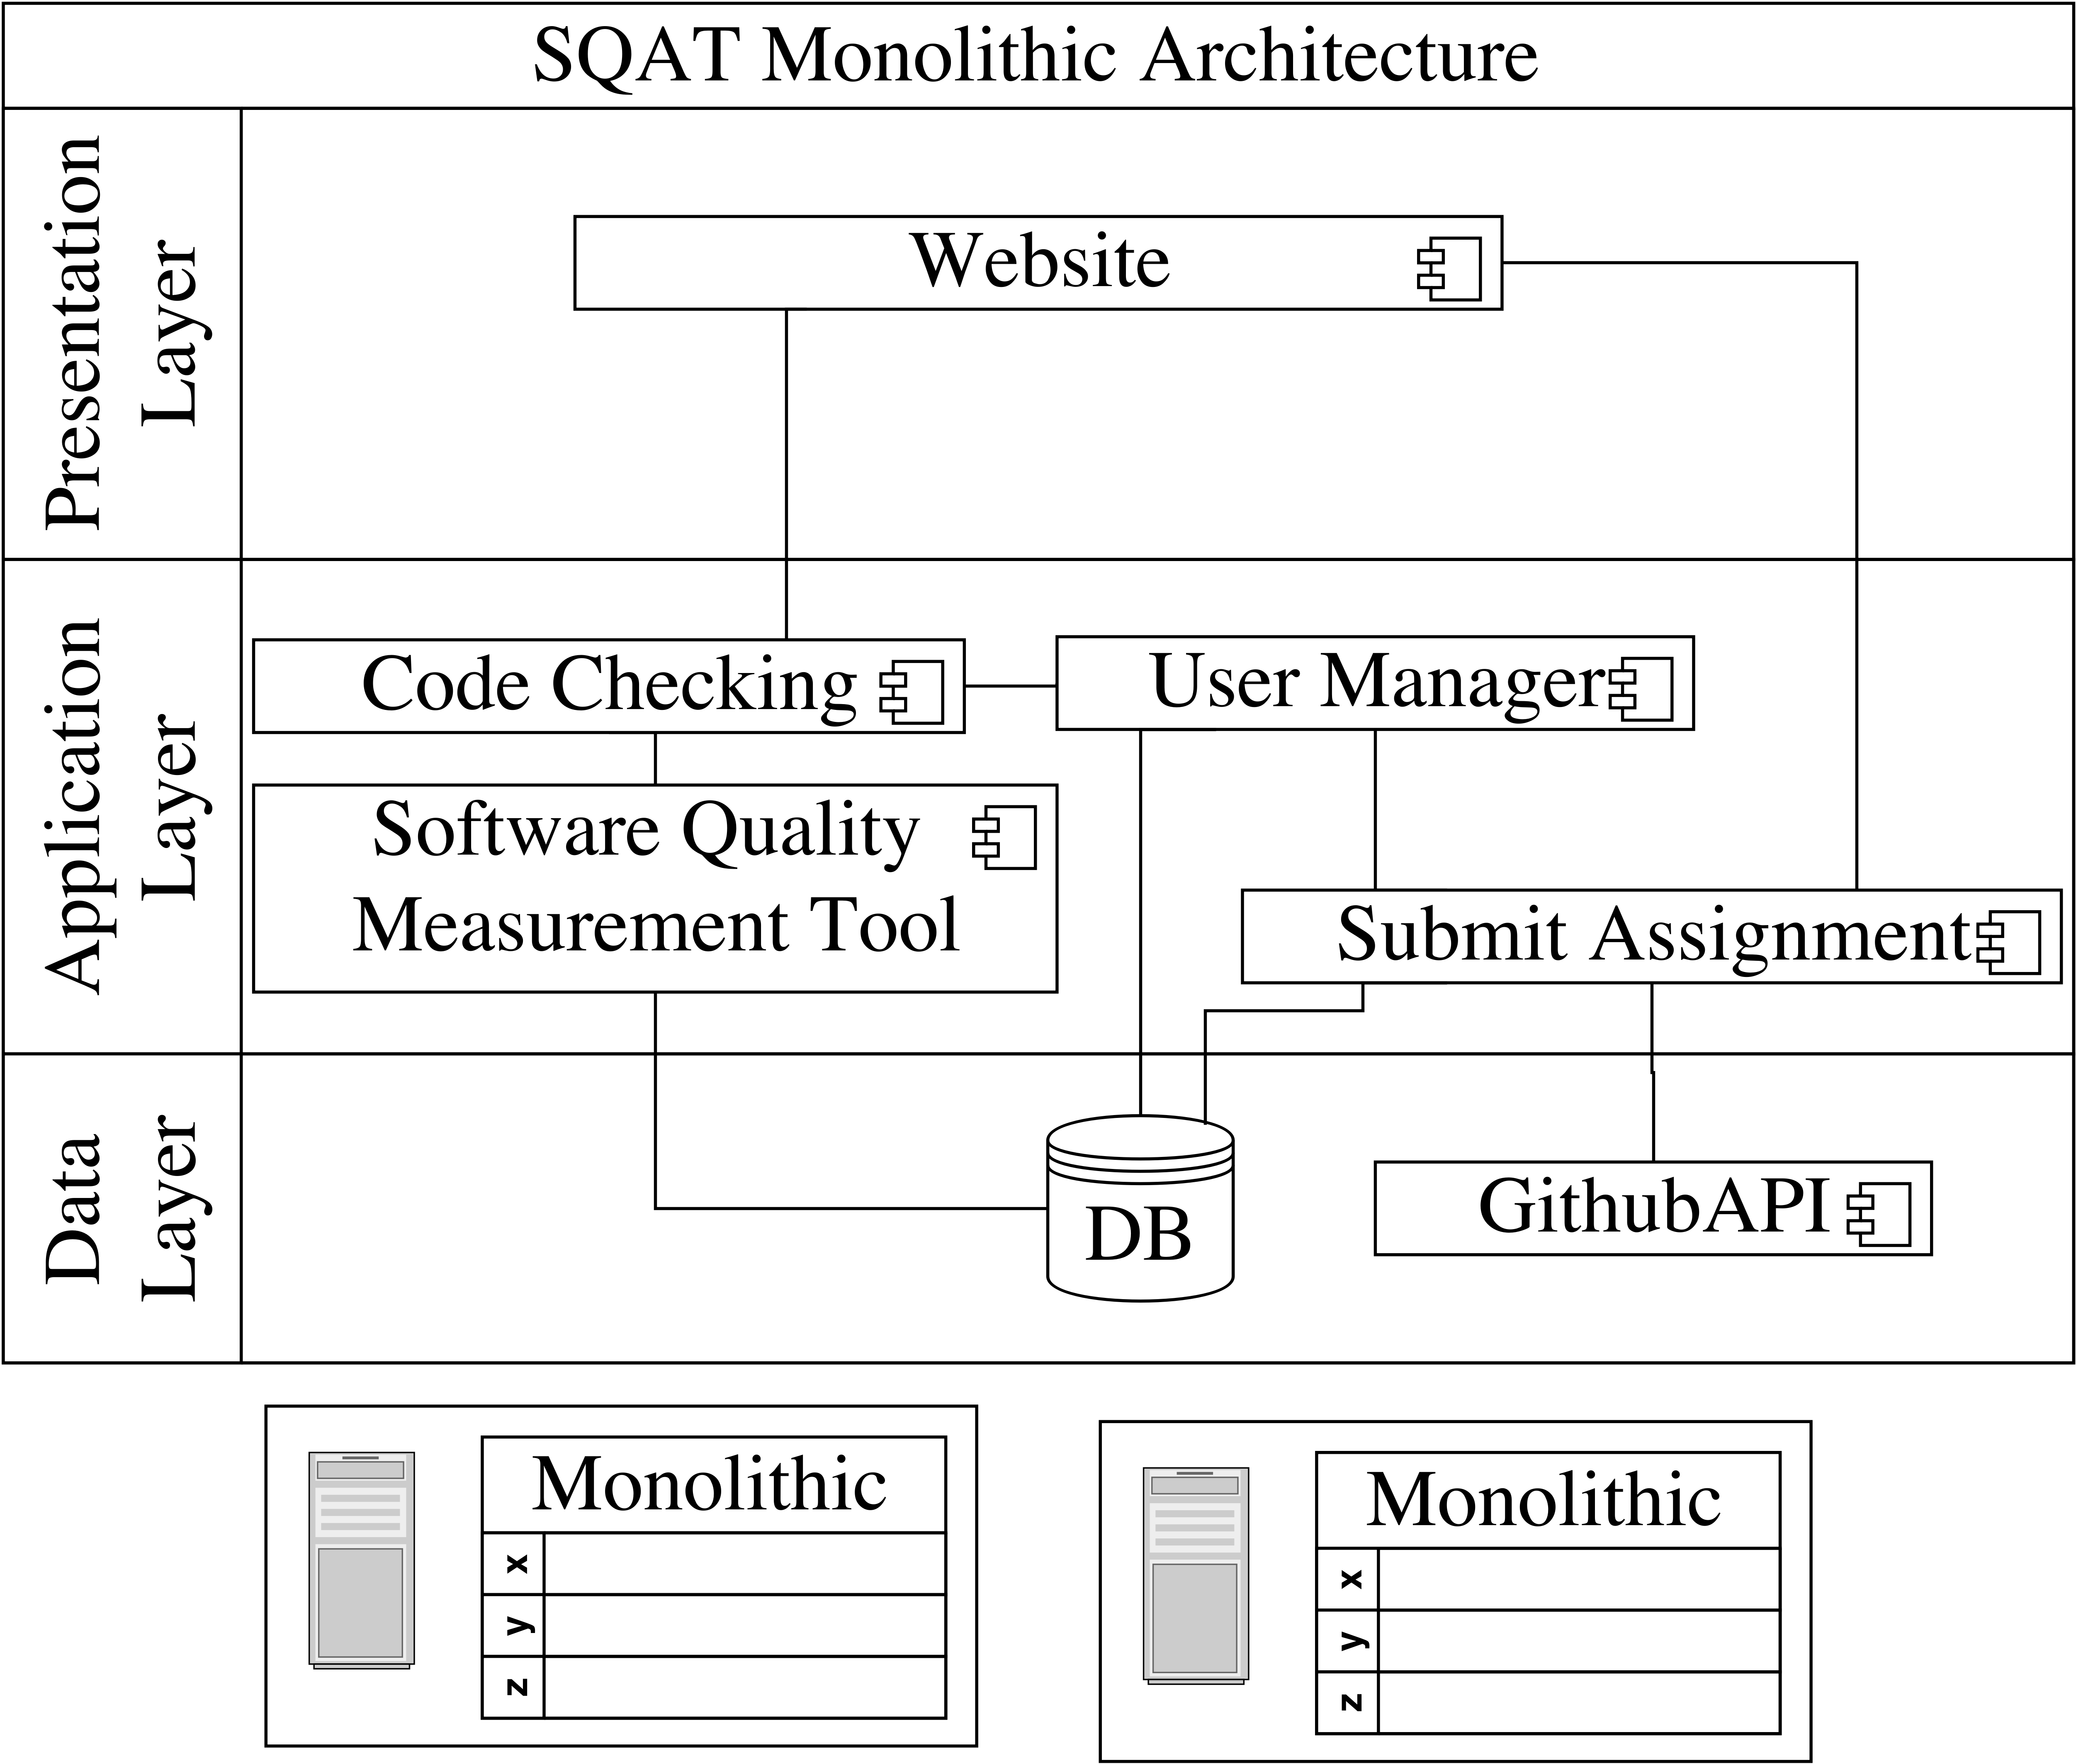
\includegraphics[width=12cm]{SQAT_monolithic.png}
    \caption{Multi-tier architecture for SQAT}
    \label{figure:SQAT_monolithic}
\end{figure}

Considering the disadvantages of monotolithic architecture, we decided to use microservice architecture for SQAT, as shown in Figure \ref{figure:microservices_architecture}. The first obvious advantage of microservice architecture is that it is programming language agnostic \cite[]{martinfowler2015}. A service written in Go programming language can be used and consumed by another service written in Javascript. Although we can write every functionality in just one programming language, it would be nice if we can write each function in a chosen programming language, because each programming language has its own set of advantages and disadvantages \cite[]{prechelt2000empirical}. We list some examples here:

\begin{enumerate}
    \item The software quality measurement component should be written in Java because ANTLR parser provide a nice API in Java.
    \item We should use programming language that provides most of the essential tools to develop a web server, such as Node.js, Python and Go. 
    \item Front-end web application should be written in Javascript and HTML
\end{enumerate}

By using microservices architecture, we can scale our application horizontally at service level \cite[]{martinfowler2015}, as shown at the bottom of Figure \ref{figure:microservices_architecture}. For example, we can use more servers to host software quality measurement service to solve the problem we present at the beginning of this chapter. By doing so, we can serve more requests while using the most optimised number of servers. Abstraction at service level also allows new developers to understand and learn the whole system faster. New developers only need to understand the APIs provided by services in order to use these services. 

\begin{figure}[t]
    \centering
    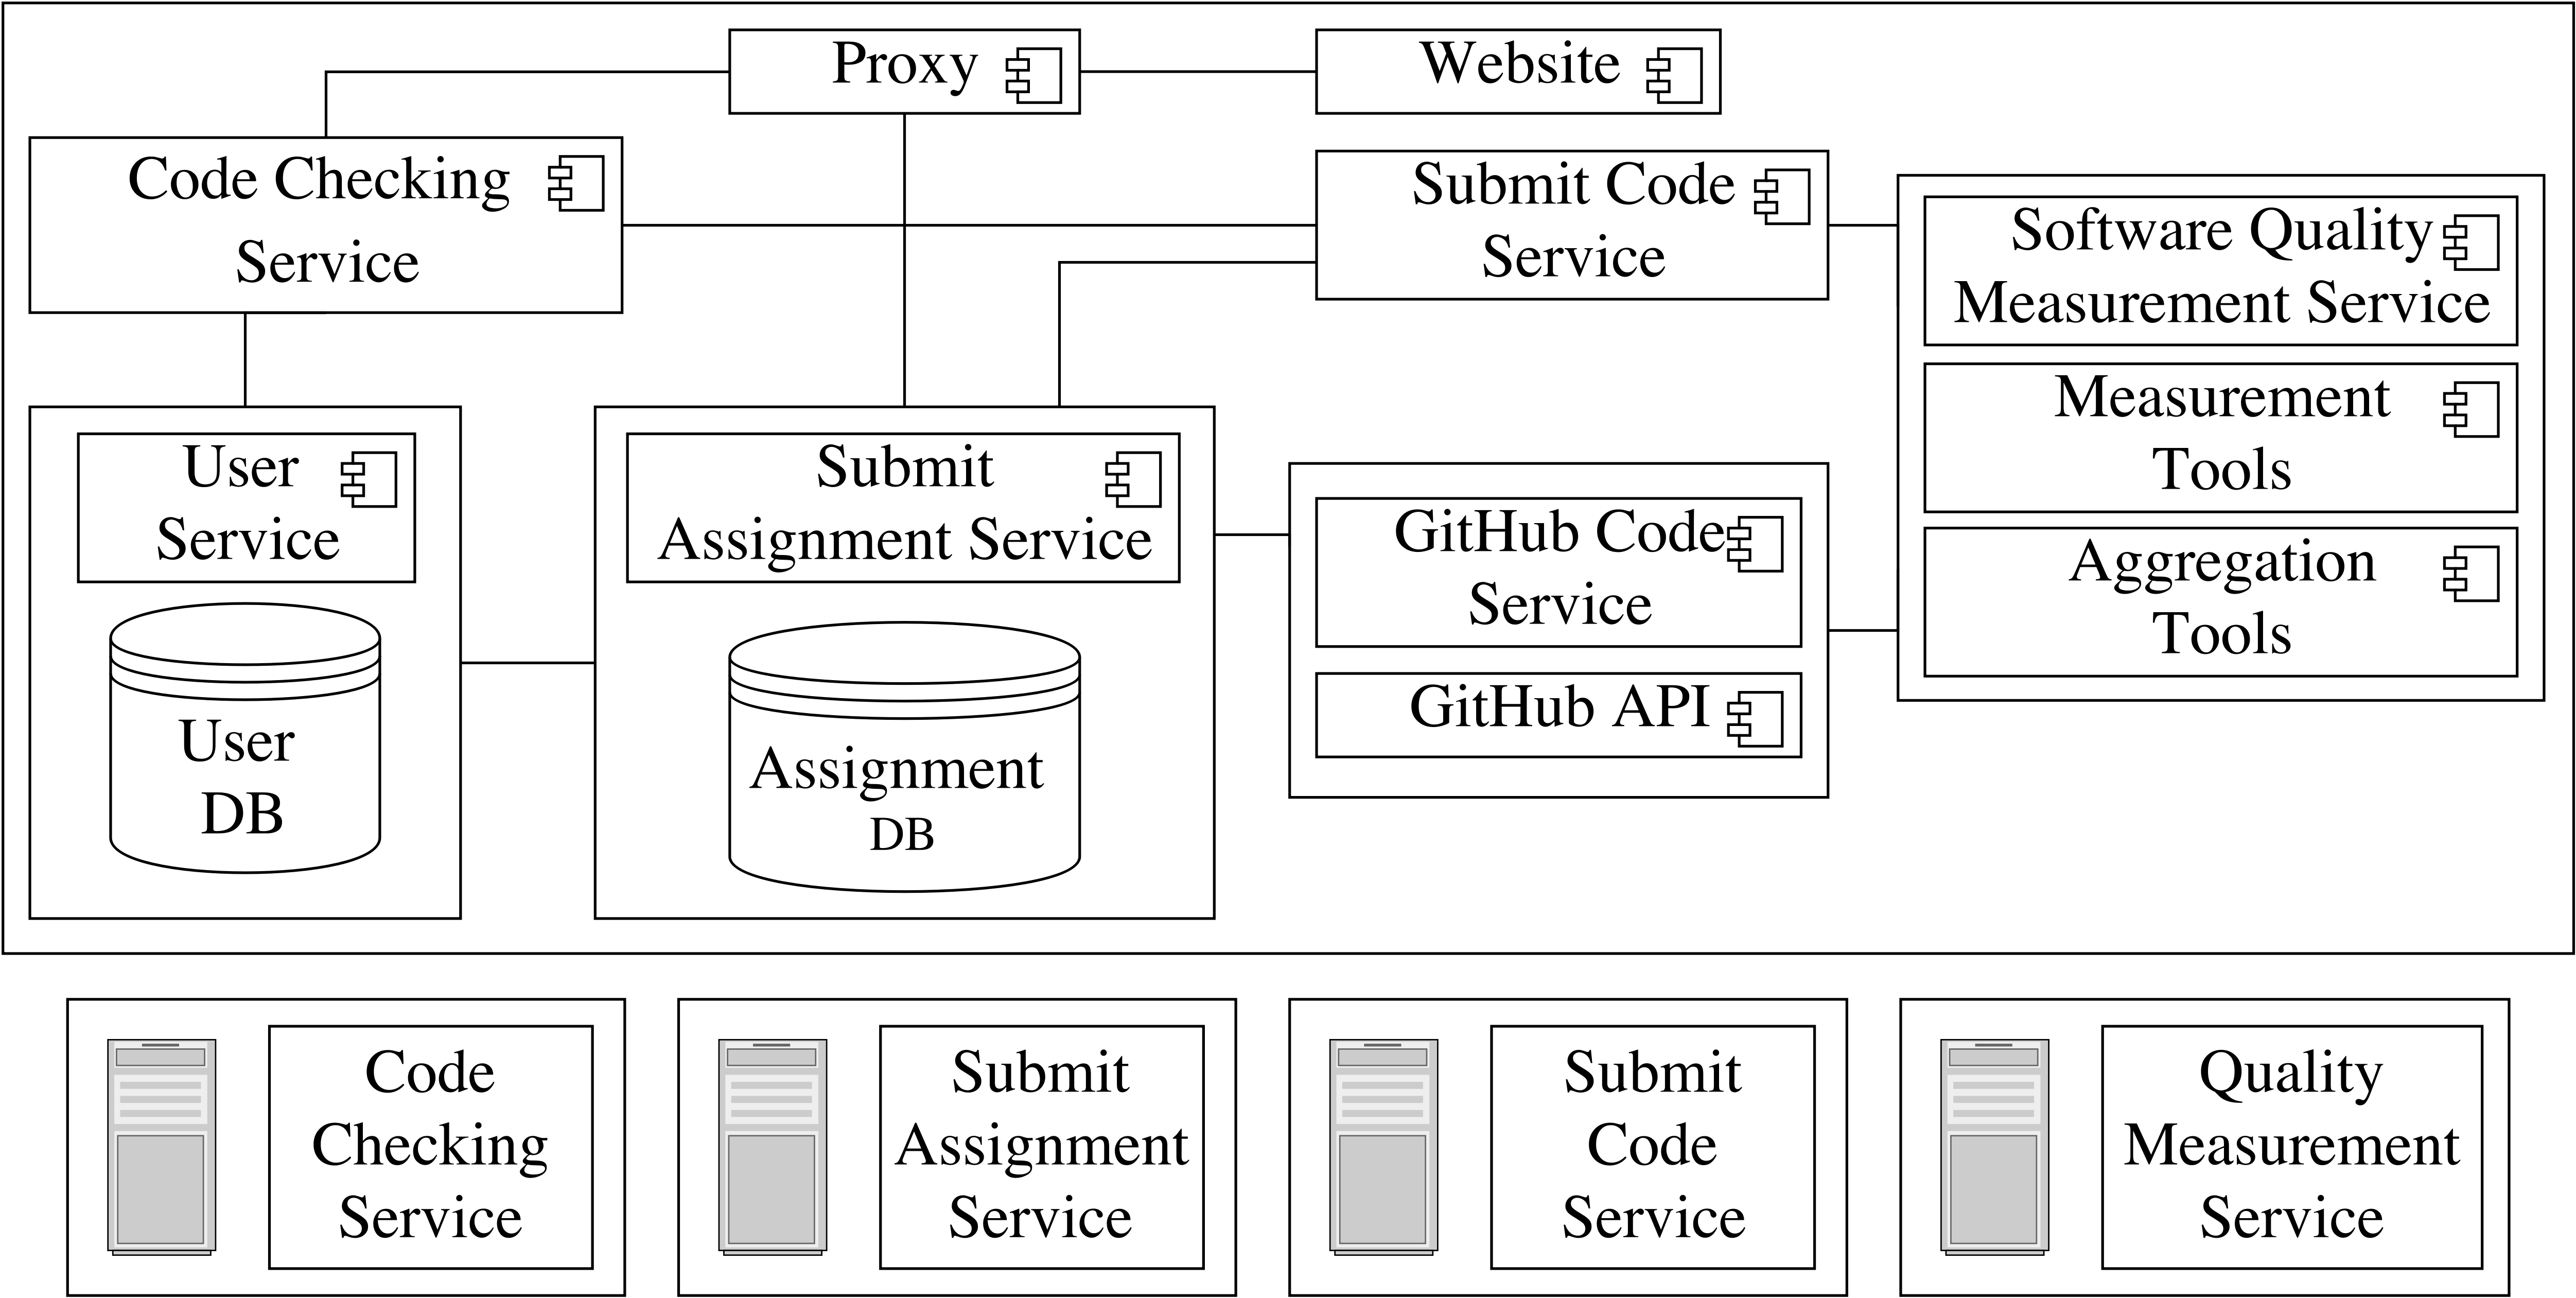
\includegraphics[width=14cm]{microservice_architecture.png}
    \caption{Microservices architecture for SQAT}
    \label{figure:microservices_architecture}
\end{figure}

% We used microservices architecture style in SQAT. The Unified Modeling Language (UML) diagram in Figure \ref{figure:microservices_architecture} shows the four main components for SQAT, i.e. proxy, website, submit code service and software quality measurement service. The website component is self-explanatory. It serves a static web user interface. The software quality measurement service measures software quality attribute quantitatively and checks for consistent code style. Submit code service acts as a middleman between client requests and software quality measurement service and can be used to perform many tasks, such as user management and errors checking before forwarding requests to software quality measurement service component. Proxy is the main point of contact between client requests and SQAT. It forwards user requests to related components using the following rules:

% \begin{enumerate}
%     \item If the Uniform Resource Locator (URL) path start with \verb|/submitSourceCode|, then route the request to submit code service.
%     \item Else, route the request to website component which serves static contents.
% \end{enumerate}

The connectors between services Figure \ref{figure:microservices_architecture} are language-agnostic APIs. Specifically, we use GRPC, a remote procedure call (RPC) library developed by Google. We will discuss GRPC in details in the next section. 

\subsection{GRPC and Protocol Buffer}

GRPC allows us to do RPC from 7 programming languages \cite[]{mugurmarculescu2015} \footnote{At the point of writing, GRPC supports C++, C\#, Objective C, Java, Go, NodeJS, Python, PHP, and Ruby}, which means that we can write a function call in Java to call for another function written in Go. GRPC uses Protocol Buffer to serialise structure data in a language agnostic way. 

We show an example to demonstrate the usage of GRPC in SQAT. Let say we want to define a RPC between software quality measurement service component and submit source code service component. First, we need to define the message structures and the RPC in Protocol Buffer definition (.proto) file as shown in Figure \ref{figure:proto_rpc}. We define \verb|StyleCheck| service that provide a RPC named \verb|Check|. The \verb|Check| method accept \verb|StyleCheckRequest| as argument and return \verb|StyleCheckReply|. The definitions of the argument and return types are included in Appendix \ref{appendix:protocol_buffer}. This definition file cannot be used directly by any programming language. Instead, we use GRPC library to consume these information. By doing so, we can do RPC from one component to another component. 

\begin{figure}[t]
\begin{minted}
[frame=single,baselinestretch=1.0,fontsize=\footnotesize]
{python}
service StyleCheck {
  rpc Check (StyleCheckRequest) returns (StyleCheckReply) {}
}
\end{minted}
\caption{An example of a RPC definition in a .proto file}
\label{figure:proto_rpc}
\end{figure}

\section{ANTLR}

ANTLR (ANother Tool for Language Recognition) is a powerful parser generator for reading, processing, executing, or translating structured text or binary files \cite[]{parr2013definitive}. From a grammar, ANTLR generates a parser that can build and walk parse trees. In SQAT, we use ANTLR to collect metrics from Java codes in software quality measurement service. We need to first define Java language structure in a grammar file, which will be accepted by ANTLR. However, defining Java language by ourselves would be tedious. Instead, we use an open source Java language definition for Grammar-V4 project \footnote{The project is hosted in GitHub: https://github.com/antlr/grammars-v4}. Next, we use Gradle\footnote{Gradle is a general purpose build tools in Java world. Although we didn't mention it in this report, we use Gradle extensively for our Java project. } and ANTLR plug-in for Gradle to generate \verb|JavaLexer|, \verb|JavaParser| and \verb|JavaListener|. These classes would be familiar to readers who have understanding in compiler techniques. 

To analyse and collect metrics from a piece of Java code, we will use the \verb|JavaLexer| to generate a stream of tokens and use \verb|JavaParser| to generate a parse tree. We will use \verb|ParseTreeWalker| to traverse the generated parse tree. While traversing the parse tree, the walker will inform a \verb|JavaListener|, which is defined by us. 

\verb|JavaListener| has 204 methods that will be called when the walker performs certain actions. Some examples of these methods are \verb|enterMethodDeclaration()| and \verb|exitMethodDeclaration()|. For example, if we want to count the number of methods in a piece of Java code, we would override the \verb|enterMethodDeclaration()| method and increment a counter when the method is called by the tree walker. By using ANTLR, we can collect all software quality metrics. 

\section{Architecture of Software Quality Measurement Component} \label{section:architecture_of_sqat_core}

Software quality measurement component is the core component for SQAT. It measures software quality attributes quantitatively using Goal Question Metric (GQM) paradigm. We use the framework proposed by \cite{washizaki2007framework} to build the component. We can observe a clear mapping from the proposed framework as shown in Figure \ref{figure:washizaki_framework}, to the structure software quality measurement component in Figure  \ref{figure:software_quality_framework}. Specifically, the measurement tool in proposed framework is mapped to ANTLR, which is a tool we used in SQAT to extract quality metrics from given source code. In addition, the aggregation tool is mapped to score calculator in SQAT. The score calculator do use the technique to normalize measured values (as described in original paper) to calculate score based on metrics and benchmarks. However, it only allow evaluation of score at component level, which is different from the original aggregation tool that allows evaluation from the component level up to whole system. Finally, the visualisation tool is mapped to a web component in SQAT, which will show the result in a single page application. The rating level deriving tool, originally presents in the \cite{washizaki2007framework} paper, is not implemented in SQAT. The tool could be something to be done in the future, which will be described in details in section \ref{section:future_recommendation}. Since we do not implement the tool in SQAT, the benchmark values (output of the tool) is just some test values.

\begin{figure}[t]
    \centering
    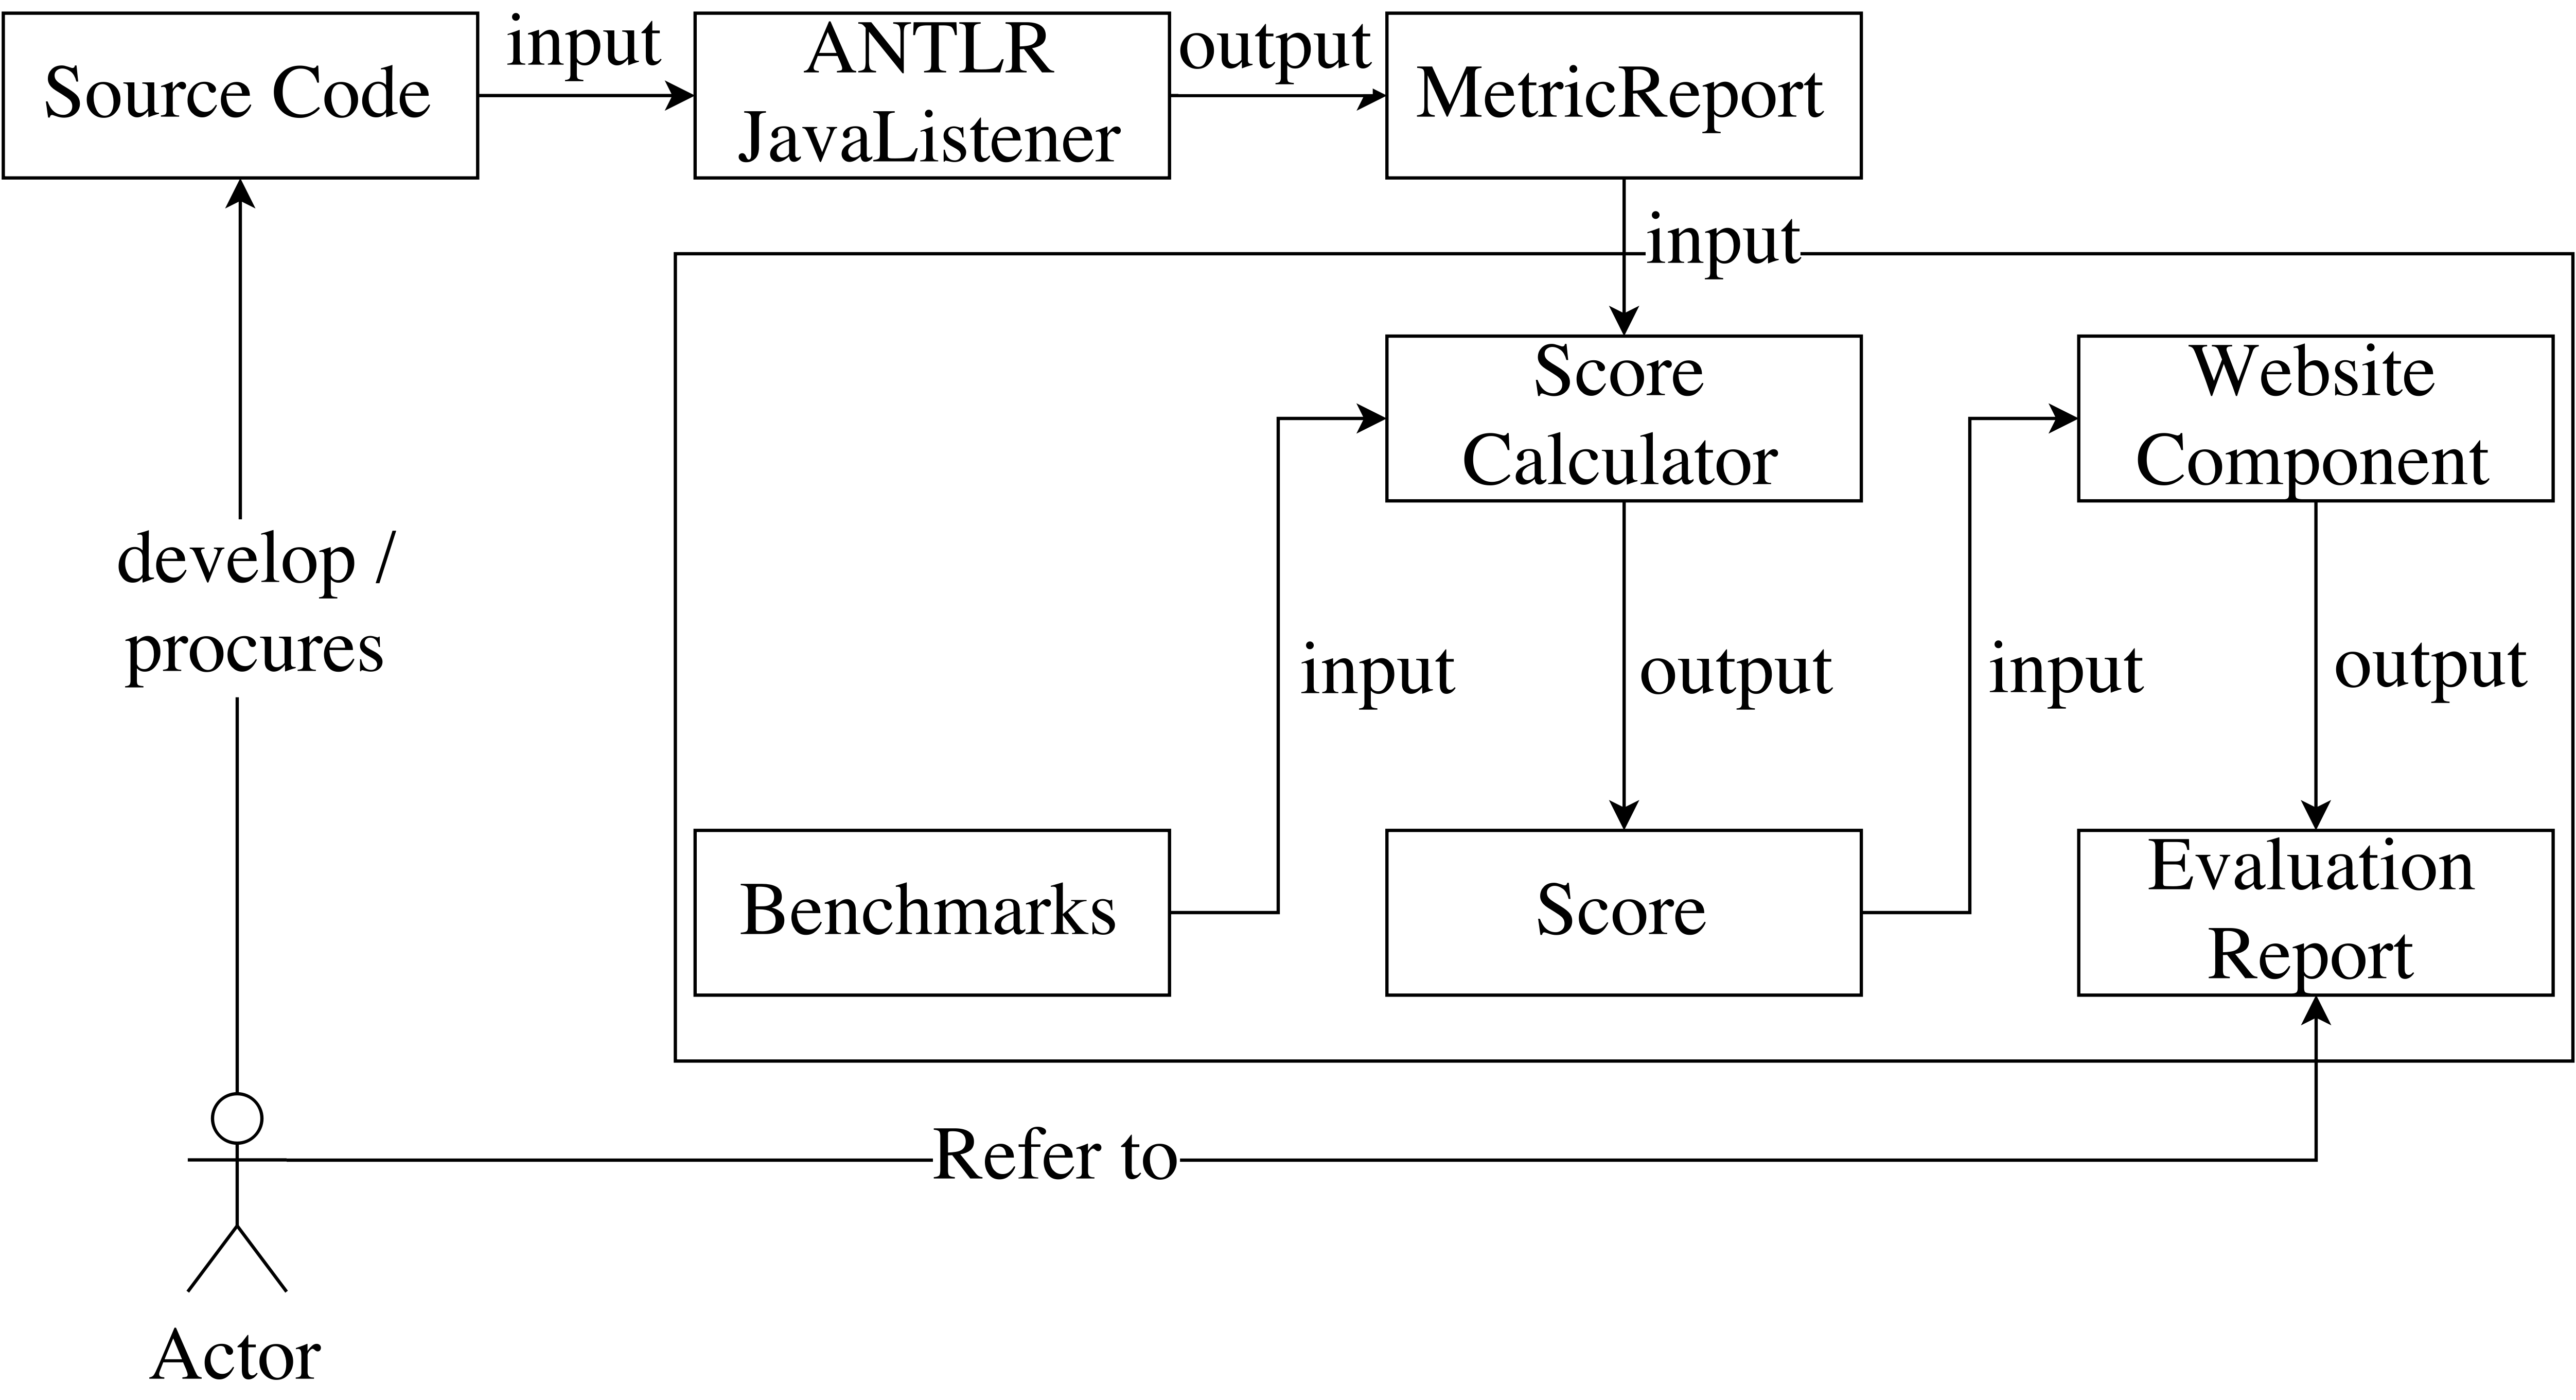
\includegraphics[width=14cm]{software_quality_measurement_framework.png}
    \caption{Structure of the SQAT software quality measurement component.}
    \label{figure:software_quality_framework}
\end{figure}

We use GQM to build a quality metric suite. In the initial version of SQAT, we define 2 goals and 5 number of question and metric pairs. The quality metric suite is shown in Table \ref{table:gqm}. This quality metric suite will be used by score calculator (aggregation tool) to calculate score for a given source codes. The details calculation will be discussed in section \ref{section:score_calculator}

\begin{table}
\centering
\begin{tabular}{| l | p{6cm}| p{4cm} |}
    \hline
    Goal & Question & Metrics \\
    \hline
    Analysability & Is the size of the code not too large? & Line of codes \\
    & Are the conditional statements not deep? & Depth of conditional nesting \\
    & Are the naming of variables good? & Average length of identifier \\
    & Are classes too complicated? & Number of Attributes \\
    & Are classes too complicated? & Number of Methods \\
    \hline
    Testability & Is the size of the code not too large? & Line of codes \\
    & Are the conditional statements not deep? & Depth of conditional nesting \\
    \hline
\end{tabular}
\caption{Using GQM to build quality metric suite}
\label{table:gqm}
\end{table} 

\section{Flux Architecture} \label{section:flux_architecture}

In traditional web page navigation, a full page refresh is made whenever you navigate to another pages / links. To improve user experience, single page application (SPA) is proposed \cite[]{mesbah2007migrating}. When we navigate in a single page application, the contents of the application is loaded dynamically (using Javascript), and the URL in the address bar is changed to emulate traditional navigation \cite[]{mikowski2013single}. We decided to build a SPA for SQAT front-end website. 

A single page application is typically built by using Model View Controller (MVC) architecture or Model View View Model (MVVM) architecture. However, as the application scale, MVC and MVVM architectures started to have problems. Facebook engineers have discovered the problem; When an action trigger the controller to change the state of many models, the state of the models will be reflected on many views. As a result, the change of views will trigger more actions and more models will be changed \cite[]{jingchen2014}. When an application is small, this is the typical way that views get latest updates from the models. It is called two-way binding \cite[]{heinrich2011websoda}. However, when an application grows, two-way binding creates infinite loops in MVC architecture, as shown in Figure \ref{figure:mvc_problems}. 

\begin{figure}[t]
\centering
\begin{tikzpicture}[
squarednode/.style={rectangle, draw=black!60, very thick, minimum size=1cm},
]
%Nodes
\node[squarednode](action){Action};
\node[squarednode](controller)[right=of action]{Controller};

\node[squarednode](model1)[right=of controller]{Model};
\node[squarednode](model2)[above=of model1]{Model};
\node[squarednode](model3)[below=of model1]{Model};

\node[squarednode](view1)[right=of model1]{View};
\node[squarednode](view2)[above=of view1]{View};
\node[squarednode](view3)[below=of view1]{View};

%Lines
\draw[->] (action.east) -- (controller);

\draw[->] (controller.east) -- (model1.west);
\draw[->] (controller.east) -- (model2.west);
\draw[->] (controller.east) -- (model3.west);

\draw[->] (model1.east) -- (view1.west);
\draw[->] (model2.east) -- (view2.west);
\draw[->] (model3.east) -- (view3.west);

\draw[->] (model2.east) -- (view3.west);
\draw[->] (model3.east) -- (view2.west);

\draw[->] (view1.west) -- (model2.east);
\end{tikzpicture}
\caption{Traditional MVC architecture creates infinite loops when the number of models and views increase.}
\label{figure:mvc_problems}
\end{figure}

To solve the problem, Facebook has proposed a solution called Flux Architecture, as shown in Figure \ref{figure:flux_architecture}. Flux is a system architecture that promotes single directional data flow through an application \cite[]{billfisherjingchen2014}. There are four main components in Flux architecture:

\begin{enumerate}
    \item Action: allows us to trigger a dispatch to the stores and to include a payload of data
    \item Dispatcher: the central hub that manages all data flow in a Flux application. 
    \item Store: contain the application state and logic
    \item View: the user interface
\end{enumerate}

\begin{figure}[t]
\centering
\begin{tikzpicture}[
squarednode/.style={rectangle, draw=black!60, very thick, minimum size=1cm},
]
%Nodes
\node[squarednode](action){Action};
\node[squarednode](dispatcher)[right=of action]{Dispatcher};
\node[squarednode](store)[right=of dispatcher]{Store};
\node[squarednode](view)[right=of store]{View};

\node[squarednode](action2)[above=of store]{Action};

%Lines
\draw[->] (action.east) -- (dispatcher.west);
\draw[->] (dispatcher.east) -- (store.west);
\draw[->] (store.east) -- (view.west);

\draw[->] (view.north) -- (action2.east);
\draw[->] (action2.west) -- (dispatcher.north);
\end{tikzpicture}
\caption{Flux architecture}
\label{figure:flux_architecture}
\end{figure}

When the view gets updated states from the store, it can create an action to trigger changes in the store. However, the newly create action will not be propagated to the store until current view finish rendering. In addition, there is no way for the view to change the store directly. The structure of Flux architecture makes the system more predictable, and hence developers can easily find bugs and problems in the system. 

In this section, we articulate the disadvantages of MVC and MVVM architecture for web application and its solution. We decided to use Flux Architecture in SQAT website component. We use React.js as the view and Alt.js as Flux implementation library. The implementation details will be discussed in section \ref{section:frontend_development}.
